\lab{The Inverted Pendulum}{The Inverted Pendulum}
\label{lab:inverted_pendulum}

\objective{We will set up the LQR optimal control problem for the inverted pendulum and compute the solution numerically. 
% We will add a stochastic component to the system.
}


Think back to your childhood days when, for entertainment purposes, you'd balance objects: a book on your head, a spoon on your nose, or even a broom on your hand.
 Learning how to walk was likely your initial introduction to the inverted pendulum problem.

A pendulum has two rest points: a stable rest point directly underneath the pivot point of the pendulum, and an unstable rest point directly above. 
The generic pendulum problem is to simply describe the dynamics of the object on the pendulum (called the `bob').
The inverted pendulum problem seeks to guide the bob toward the unstable fixed point at the top of the pendulum. 
Since the fixed point is unstable, the bob must be balanced relentlessly to keep it upright. 

The inverted pendulum is an important classical problem in dynamics and control theory, and is often used to test different control strategies. One application of the inverted pendulum is the guidance of rockets and missiles. Aerodynamic instability occurs because the center of mass of the rocket is not the same as the center of drag. Small gusts of wind or variations in thrust require constant attention to the orientation of the rocket. 


\section*{The Simple Pendulum}
We begin by studying the simple pendulum setting. 
Suppose we have a pendulum consisting of a bob with mass $m$ rotating about a pivot point at the end of a (massless) rod of length $l$. 
Let $\theta(t)$ represent the angular displacement of the bob from its stable equilibrium.
By Hamilton's Principle, the path $\theta$ that is taken by the bob minimizes the functional 
\begin{align}
J[\theta] = \int_{t_0}^{t_1}	L,
\end{align}
where the Lagrangian $L = T - U$ is the difference between the kinetic and potential energies of the bob. 

The kinetic energy of the bob is given by $mv^2/2$, where $v$ is the velocity of the bob. 
In terms of $\theta$, the kinetic energy becomes 
\begin{align}
	\begin{split}
	T &= \frac{m}{2}v^2  = \frac{m}{2}(\dot{x}^2 + \dot{y}^2),\\
	&= \frac{m}{2}((l\cos(\theta)\dot{\theta})^2 + (l\sin(\theta)\dot{\theta})^2),\\
	&= \frac{ml^2\dot{\theta}^2}{2}.
	\end{split}
\end{align}
The potential energy of the bob is $U = mg(l-l\cos \theta)$. 
From these expressions we can form the Euler-Lagrange equation, which determines the path of the bob: 
\begin{align}
	\begin{split}
	0 &= L_{\theta} - \frac{d}{dx}L_{\dot{\theta}},\\
	&= -mgl\sin \theta - m l^2 \ddot{\theta},\\
	&= \ddot{\theta} + \frac{g}{l}\sin \theta.
	\end{split}
\end{align}
Since in this setting the energy of the pendulum is conserved, the equilibrium position $\theta = 0$ is only Lyapunov stable. When forces such as friction and air drag are considered $\theta = 0$ becomes an asymptotically stable equilibrium. 

\begin{figure}
\centering
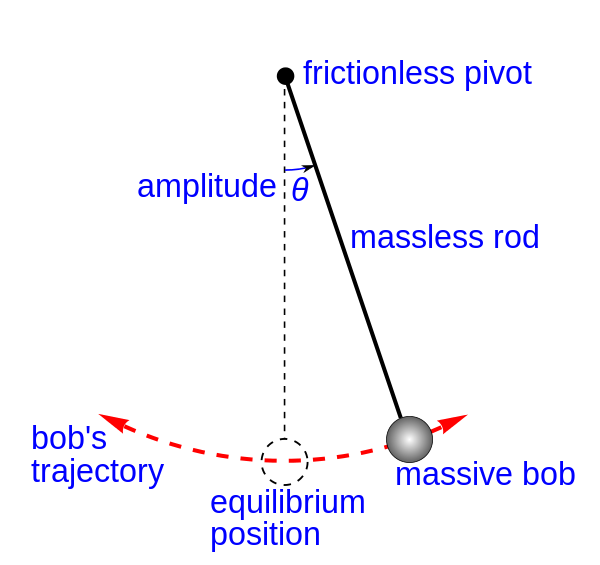
\includegraphics[width=8cm]{Simple_gravity_pendulum.png}
\caption{The frame of reference for the simple pendulum problem.
}
\label{fig:inverted_pendulum:simple_gravity_pendulum}
\end{figure}

% Let us take into account friction as a force that resists the motion of the rod about its pivot point.
% Suppose that friction is proportional to the square of the velocity of the bob: $F = -\frac{1}{2}cm(l\dot{\theta})^2$, $c > 0$.
% Recall that whenever a force field $\mathbf{F}$ has the form $\mathbf{F} = \nabla \phi(\mathbf{x})$, where $\phi(\mathbf{x})$ is a scalar field, the potential energy derived from the force of friction is $ -\phi(\mathbf{x})$. Thus introducing the force of friction requires us to modify our expression for potential energy,
% \[
% U = mg(l-l\cos \theta) + k\theta
% \]
% leading to the Euler-Lagrange equation.

% The simple pendulum problem can be modelled by the equation
% \begin{align}
%
% \end{align}



\section*{The Inverted Pendulum}
\subsection*{The Control System}
We consider a gift suspended above a rickshaw by a (massless) rod of length $l$. 
The rickshaw and its suspended gift will have masses $M$ and $m$ respectively, $M > m$.  
Let $\theta $ represent the angle between the gift and its unstable equilibrium, with counterclockwise orientation. 
Let $v_1$ and $v_2$ represent the velocities of the rickshaw and the gift, and $F$ the force exerted on the rickshaw. 
The rickshaw will be restricted to traveling along a straight line (the $x$-axis). 

By Hamilton's Principle, the path $(x,\theta)$ of the rickshaw and the present minimizes the functional 
\begin{align}
J[x,\theta] = \int_{t_0}^{t_1}	L,
\end{align}
where the Lagrangian $L = T - U$ is the difference between the kinetic energy of the present on the pendulum, and its potential energy.

Since the position of the rickshaw and the present are $(x(t),0)$ and $(x-l\sin \theta, l\cos \theta)$ respectively, the total kinetic energy is 
\begin{align}
	\begin{split}
	T &= \frac{1}{2}Mv_1^2 +  \frac{1}{2}mv_2^2,\\
	&= \frac{1}{2}M\dot{x}^2 +  \frac{1}{2}m((\dot{x} - l\dot{\theta}\cos \theta)^2 + (- l\dot{\theta}\sin \theta)^2),\\
	&= \dot{x}^2 + l^2\dot{\theta}^2-2l\dot{x}\dot{\theta}\cos \theta.
	\end{split}
\end{align}
% The potential energy $U$ is composed of two parts: the first is the gravitational potential energy of the bob/present on the pendulum, and is given by $(mg)(l\cos \theta)$.
% The second part is the potential energy in the system due to any force $F$ exerted on the rickshaw.
% Recalling that whenever a force field $\mathbf{F}$ has the form $\mathbf{F} = \nabla \phi(\mathbf{x})$, where $\phi(\mathbf{x})$ is a scalar field, the potential energy derived from that force is $ -\phi(\mathbf{x})$.
The total potential energy is 
\begin{align*}
U &= mgl\cos \theta - Fx.
\end{align*}

\begin{figure}
\centering
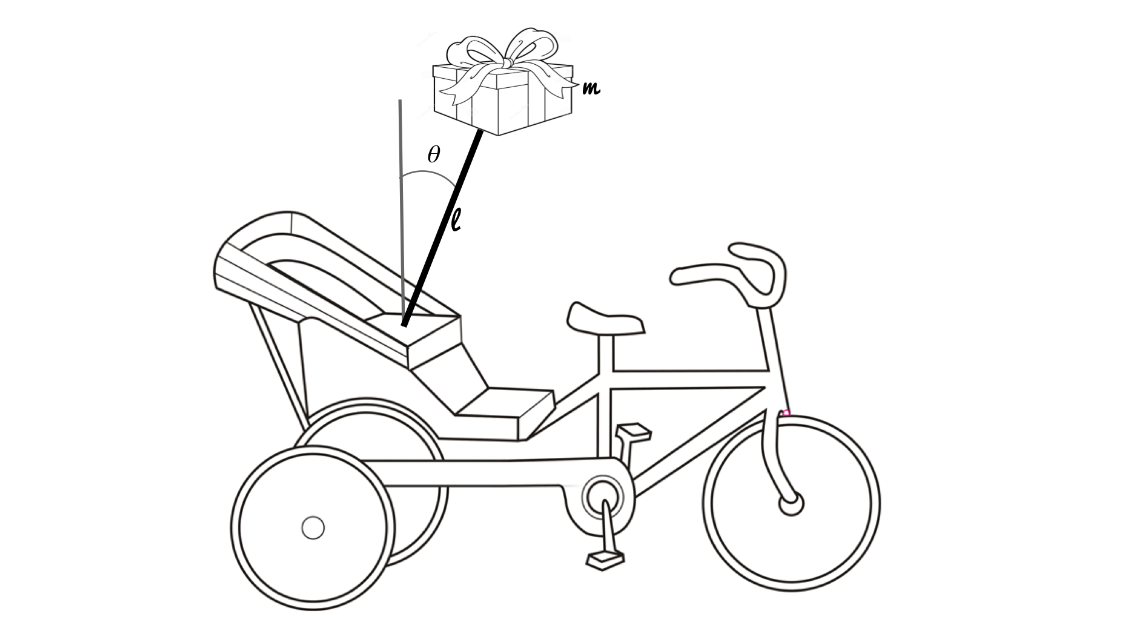
\includegraphics[width=\textwidth]{rickshaw_img.png}
\caption{The inverted pendulum problem on a mobile rickshaw with a present suspended above.
}
\label{fig:inverted_pendulum:rickshaw_diagram}
\end{figure}

% Pulling these expressions together, we see that the functional $J$ is given by
% \begin{align}
% 	J[x,\theta] = \int_{t_0}^{t_1} \frac{1}{2}Mv_1^2 +  \frac{1}{2}mv_2^2 - mgl\cos \theta + Fx,
% \end{align}
Since the path $(x,\theta)$ of the rickshaw and the present satisfy the Euler-Lagrange differential equations 
\begin{align}
	\begin{split}
\frac{\partial L}{\partial x} - \frac{d}{dt} \frac{\partial L}{\partial \dot{x}} &= 0,\\
\frac{\partial L}{\partial \theta} - \frac{d}{dt} \frac{\partial L}{\partial \dot{\theta}} &= 0,
	\end{split}\label{inverted_pendulum:langrange_eqns}
\end{align}
after expanding \eqref{inverted_pendulum:langrange_eqns} we see that $x(t)$ and $\theta(t)$ satisfy
\begin{align}
	\begin{split}
		F &= (M + m)\ddot{x} - ml\ddot{\theta} \cos \theta + ml \dot{\theta}^2 \sin \theta,\\
		l \ddot{\theta} &= g \sin \theta + \ddot{x} \cos \theta.
	\end{split}\label{inverted_pendulum:langrange_eqns_explicit}
\end{align}



At this point we make a further simplifying assumption. 
If $\theta$ starts close to $0$, we may assume that the corresponding force $F$ will keep $\theta$ small. 
In this case, we linearize \eqref{inverted_pendulum:langrange_eqns_explicit} about $(\theta, \dot{\theta}) = (0,0)$, obtaining the equations 
\begin{align*}
	\begin{split}
		F &= (M + m)\ddot{x} - ml\ddot{\theta},\\
		l \ddot{\theta} &= g \theta + \ddot{x}.
	\end{split}%\label{inverted_pendulum:langrange_eqns_explicit2}
\end{align*}
These equations can be further manipulated 
 % \eqref{inverted_pendulum:langrange_eqns_explicit2}
to obtain 
\begin{align}
	\begin{split}
		\ddot{x} &= \frac{1}{M}F - \frac{m}{M}g\theta,\\
		\ddot{\theta} &= \frac{1}{Ml}F + \frac{g}{Ml} (M+m) \theta.
	\end{split}\label{inverted_pendulum:langrange_eqns_explicit3}
\end{align}

We will now write \eqref{inverted_pendulum:langrange_eqns_explicit3} as a first order system. 
Making the assignments $x_1 = x$, $x_2 = x_1'$, $\theta_1 = \theta$, $\theta_2 = \theta_1'$, letting $u = F$ represent the control variable, we obtain 
\begin{align*}
\begin{bmatrix}
x_1\\
x_2 \\
\theta_1 \\
\theta_2
\end{bmatrix}' &= 
\begin{bmatrix}
0 & 1 & 0 & 0\\
0 & 0 & \frac{mG}{M} & 0 \\
0 & 0 & 0 & 1 \\
0 & 0 & \frac{g}{Ml}(M+m) & 0
\end{bmatrix}
\begin{bmatrix}
x_1\\
x_2 \\
\theta_1 \\
\theta_2
\end{bmatrix} + u
\begin{bmatrix}
0\\
\frac{1}{M} \\
0 \\
\frac{1}{Ml}
\end{bmatrix},
\end{align*}
which can be written more concisely as 
\[z' = Az + Bu.\]


\begin{problem}
Write a function that returns the matrices $A, B, Q$, and $R$ given above. Let $g = 9.8\text{ m}/\text{s}^2$.	
	
\begin{lstlisting}

def linearized_init(M, m, l, q1, q2, q3, q4, r): 
	'''
	Parameters:
	----------
	M, m: floats
          masses of the rickshaw and the present
	l 	: float
          length of the rod
	q1, q2, q3, q4, r : floats
         relative weights of the position and velocity of the rickshaw, the 
		 angular displacement theta and the change in theta, and the control
	
	Return
	-------
	A : ndarray of shape (4,4) 
	B : ndarray of shape (4,1) 
	Q : ndarray of shape (4,4) 
	R : ndarray of shape (1,1) 
	'''
	pass	
\end{lstlisting}
\end{problem}


\subsection*{The infinite time horizon LQR problem}
We consider the cost function
\begin{align}
\begin{split}
J[z] &= \int_0^{\infty} (q_1x_1^2 + q_2x_2^2  + q_3\theta_1^2 + q_4\theta_2^2 + ru^2)\, dt\\
&= \int_0^{\infty} z^TQz + u^TRu \, dt
\end{split} \label{inverted_pendulum:LQR}
\end{align}
where $q_1, q_2, q_3, q_4$, and $r$ are nonnegative weights, and 
\[
Q = 
\begin{bmatrix}
q_1 & 0 & 0 & 0 \\
0 & q_2 & 0 & 0\\
0 & 0 & q_3 & 0 \\
0 & 0 & 0 & q_4
\end{bmatrix}, R = \begin{bmatrix} r \end{bmatrix}.
\]
The optimal control problem \eqref{inverted_pendulum:LQR} is an example of a Linear Quadratic Regulator (LQR), and is known to have an optimal control $\tilde{u}$ described by a linear state feedback law:
\begin{align*}
\tilde{u} &= -R^{-1}B^TP\tilde{z}.
\end{align*}
Here $P$ is a matrix function that satisfies the Riccati differential equation (RDE)
\[
\dot{P}(t) = PA + A^TP + Q - PBR^{-1}B^T P.  
\]
Since this problem has an infinite time horizon, we have $\dot{P} = 0$. Thus $P$ is a constant matrix, and can be found by solving the algebraic Riccati equation (ARE)
\begin{align}
 PA + A^TP + Q - PBR^{-1}B^T P = 0.  \label{inverted_pendulum:ARE}
\end{align}
The evolution of the optimal state vector $\tilde{z}$ can then be described by \footnote{See Calculus of Variations and Optimal Control Theory, Daniel Liberzon, Ch.6}
\begin{align}
\dot{\tilde{z}} = (A - BR^{-1}B^TP)\tilde{z}. \label{inverted_pendulum:optimal_state}
\end{align}

\begin{problem}
Write the following function to find the matrix $P$. 
Use \li{scipy.optimize.root}. 
Since \li{root} takes in a vector and not a matrix, you will have to reshape the matrix $P$ before passing it in and after getting your result, using \li{np.reshape(16)} and \li{np.reshape((4,4))}.
\begin{lstlisting}
def find_P(A,B,Q,R):
	'''
	Parameters:
	----------
	A, B, Q : ndarrays of shape (4,4)
	R		: ndarray of shape (1,1)
	
	Returns
	-------
	P		: the matrix solution of the Riccati equation
	'''
	pass


\end{lstlisting}
Using the values 
\begin{lstlisting}
M, m = 23., 5.
l = 4.
q1, q2, q3, q4 = 1., 1., 1., 1.
r = 5.
\end{lstlisting}
compute the eigenvalues of $A - BR^{-1}B^TP$.
Are any of the eigenvalues positive? 
Consider differential equation \eqref{inverted_pendulum:optimal_state} governing the optimal state $\tilde{z}$. 
Using this value of $P$, will we necessarily have $\dot{\tilde{z}} \to 0$?
\end{problem}


Notice that we have no information on how many solutions \eqref{inverted_pendulum:ARE} possesses. 
In general there may be many solutions. 
We hope to find a unique solution $P$ that is \textit{stabilizing}: the eigenvalues of $A - BR^{-1}B^TP$ have negative real part. 
To find this $P$, use the function \li{solve_continuous_are} from \li{scipy.linalg}. 
This function is designed to solve the continuous algebraic Riccati equation. 

\begin{problem}
	Write the following function that implements the LQR solution described earlier.  For the IVP solver, you can use your own or you may use the function \li{ode} from \li{scipy.integrate}.
\begin{lstlisting}
def rickshaw(tv,X0,A, B, Q, R_inv, P):
	'''
	Parameters:
	----------
	tv : ndarray of time values, with shape (n+1,)
	X0 : 
	A, B, Q	: ndarrays of shape (4,4)
	R_inv	: ndarray of shape (1,1), inverse of R
	P		: ndarray of shape (4,4)
	
	Returns
	-------
	Z : ndarray of shape (n+1,4), the state vector at each time
	U : ndarray of shape (n,), the control values
	'''
\end{lstlisting}
\label{prob:inverted_pendulum3}
\end{problem}

\begin{problem}
Test the function made in Problem \eqref{prob:inverted_pendulum3} with the following inputs: 
\begin{lstlisting}
M, m = 23., 5.
l = 4.
q1, q2, q3, q4 = 1., 1., 1., 1.
r = 10.
tf = 15
X0 = np.array([-1, -1, .1, -.2])
\end{lstlisting}
Use both \li{scipy.optimize.root} and \li{solve_continuous_are} to find the matrix $P$. Compare your results. The results are plotted in Figure \ref{fig:inverted_pendulum:4}.
% and \ref{fig:inverted_pendulum:prob4_stable} respectively.
\label{prob:inverted_pendulum:4}
\end{problem}


\begin{figure}
\begin{minipage}[b]{.47\linewidth}
\centering
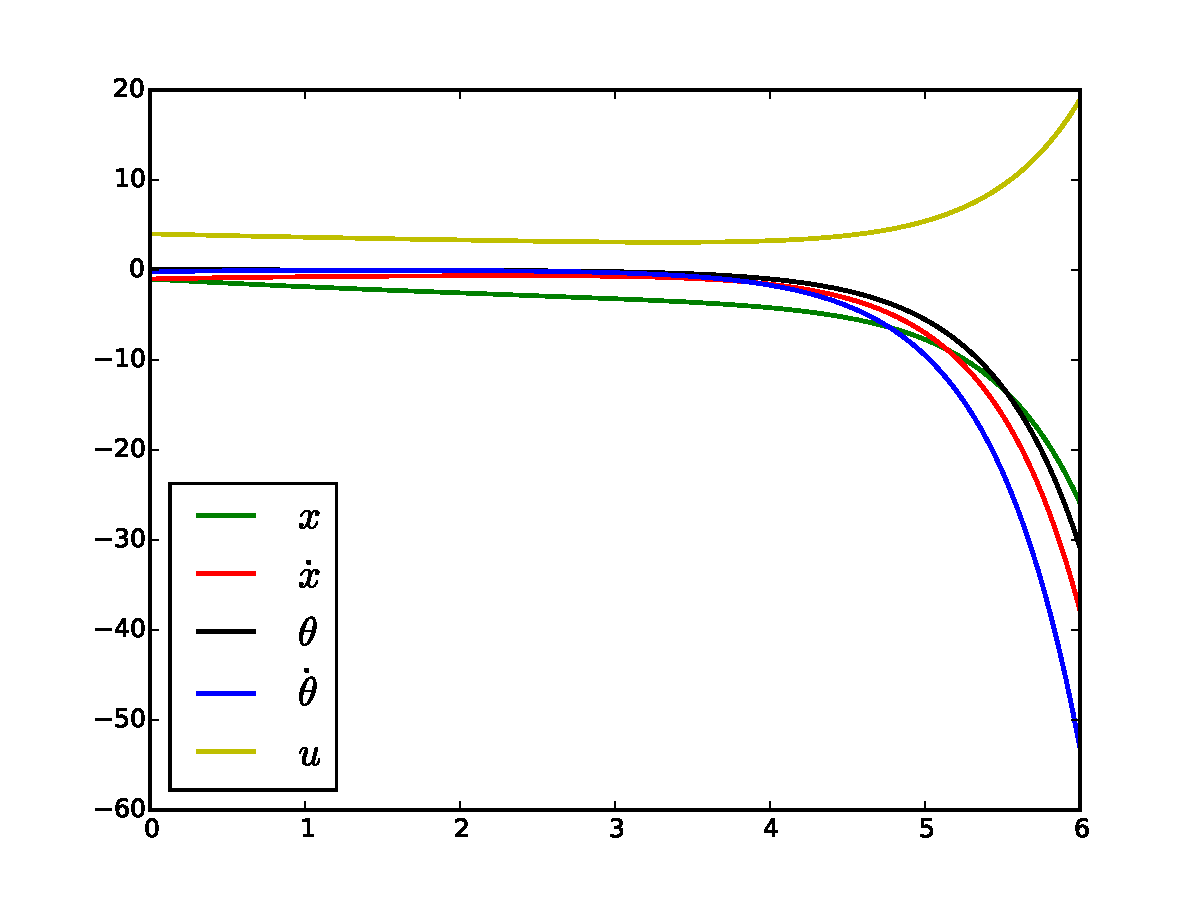
\includegraphics[width=\textwidth]{prob4_unstable.pdf}
\caption*{$P$ is found using \li{scipy.optimize.root}.}
\end{minipage}
\hspace{0.5cm}
\begin{minipage}[b]{0.47\linewidth}
\centering
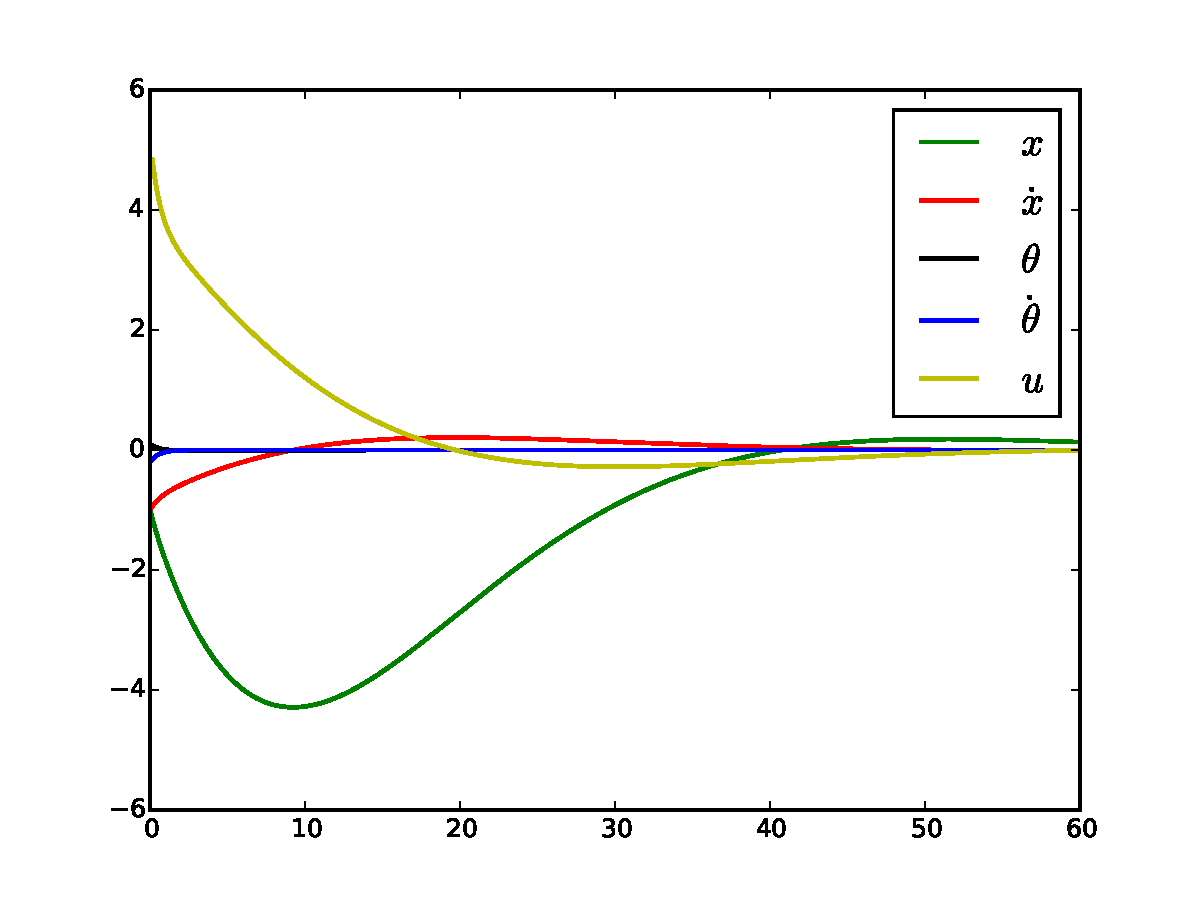
\includegraphics[width=\textwidth]{prob4_stable.pdf}
\caption*{$P$ is found using \li{solve_continuous_are}.}
\end{minipage}
\caption{The solutions of Problem \ref{prob:inverted_pendulum:4}.}
\label{fig:inverted_pendulum:4}
\end{figure}



\begin{problem}
Consider the following inputs: 
\begin{lstlisting}
M, m = 23., 5.
l = 4.
q1, q2, q3, q4 = 1., 1., 1., 1.
r = 10.
tf = 60
X0 = np.array([-1, -1, .1, -.2])
\end{lstlisting}
Vary the entries of \li{X0} responsible for $\theta(0)$ and $\dot{\theta}(0)$ to determine the sensitivity of the control $u$ to the initial conditions.  What initial conditions lead to a reasonable, physical control $u$?
\end{problem}

%
% \begin{figure}
% \centering
% 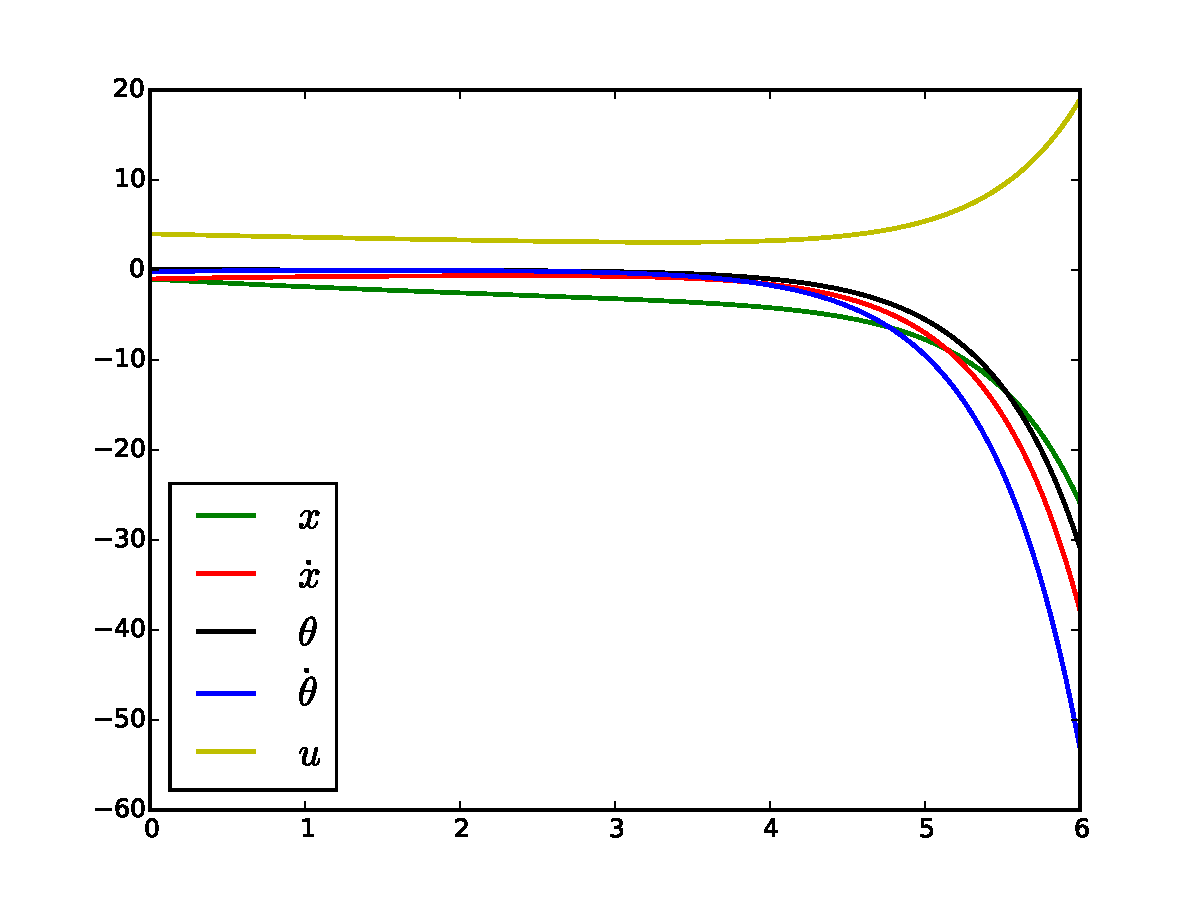
\includegraphics[width=7cm]{prob4_unstable.pdf}
% \caption{The solution of Problem \ref{prob:inverted_pendulum:4} when $P$ is found using \li{scipy.optimize.root}.
% }
% \label{fig:inverted_pendulum:prob4_unstable}
% \end{figure}
%
%
%
% \begin{figure}
% \centering
% 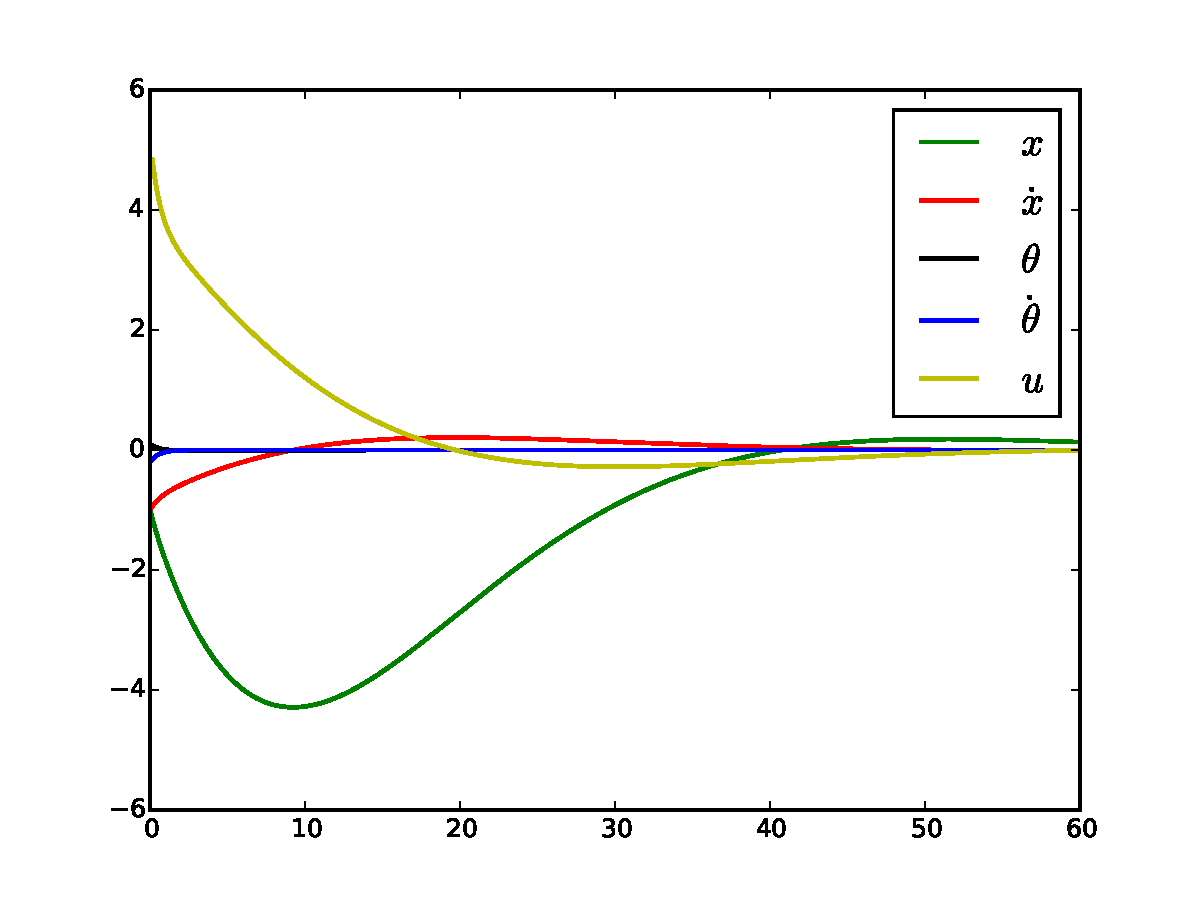
\includegraphics[width=7cm]{prob4_stable.pdf}
% \caption{The solution of Problem \ref{prob:inverted_pendulum:4} when $P$ is found using \li{solve_continuous_are}.
% }
% \label{fig:inverted_pendulum:prob4_stable}
% \end{figure}
%
%



